\subsection{字与字节}
\begin{figure}[H]
    \centering
    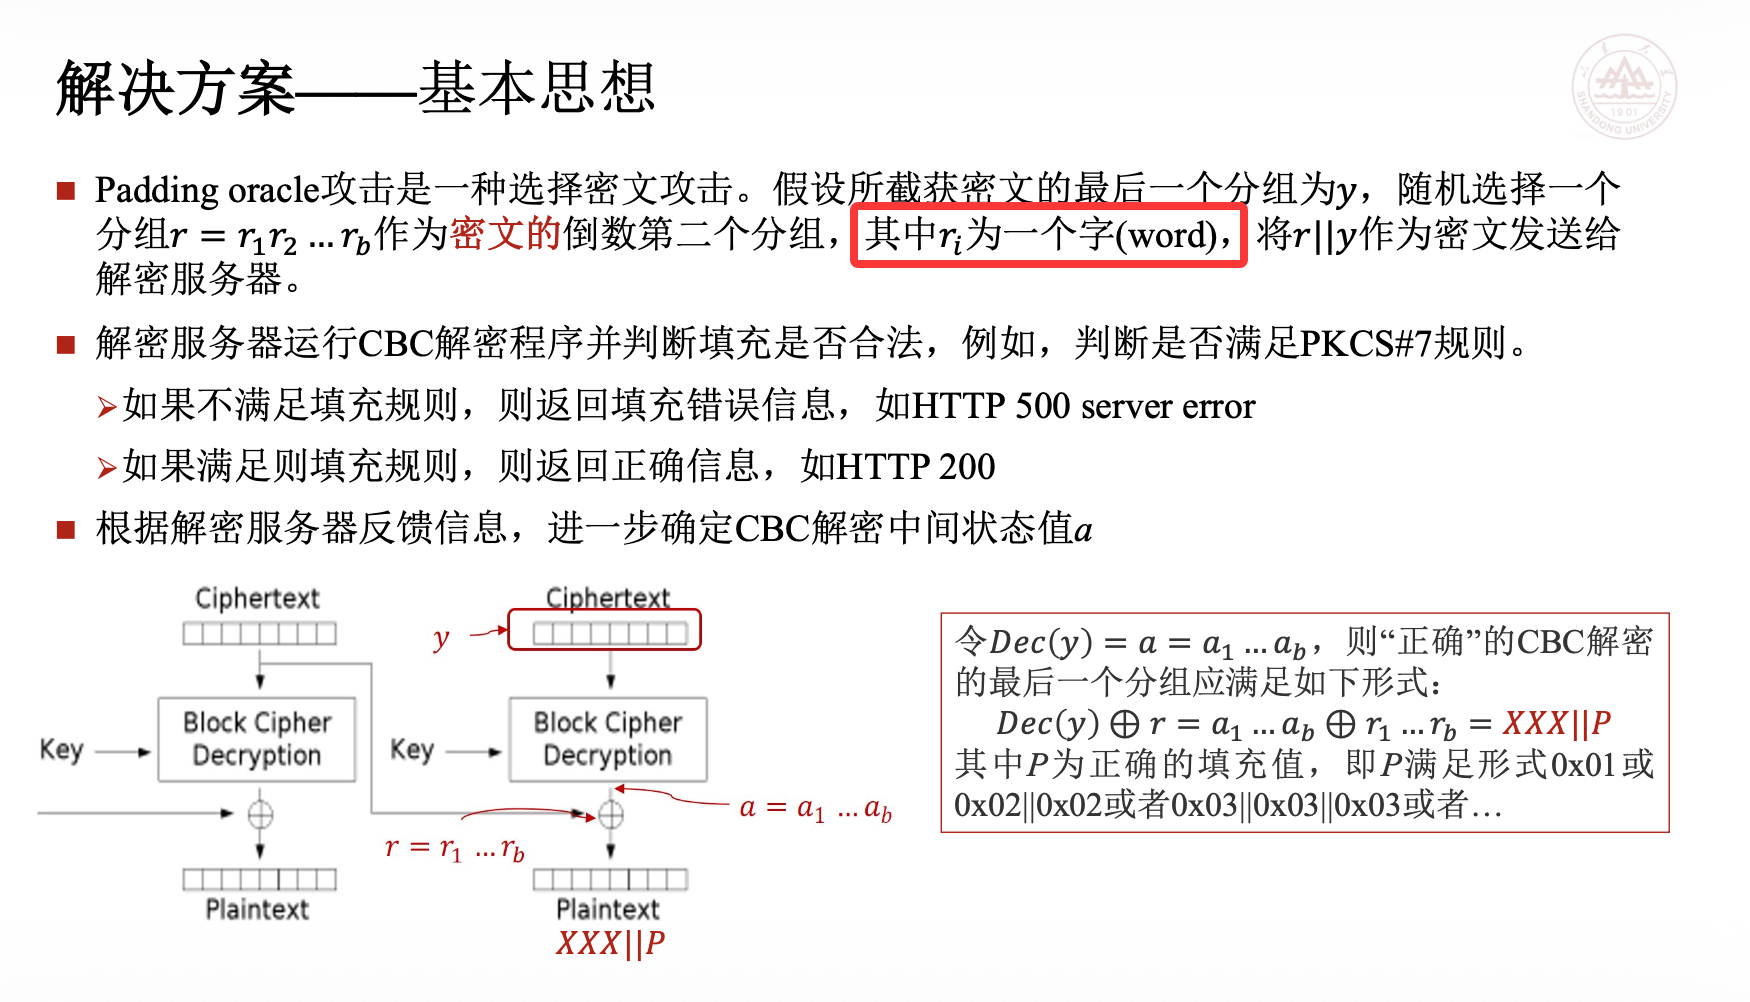
\includegraphics[width = 0.8\textwidth]{figures/error1.png}
    \caption{错误1}
\end{figure}
此处 \(r_i\) 表示的是一个字节（Byte），不是一个字（word）。
\subsection{没有必要的步骤}
\begin{figure}[H]
    \centering
    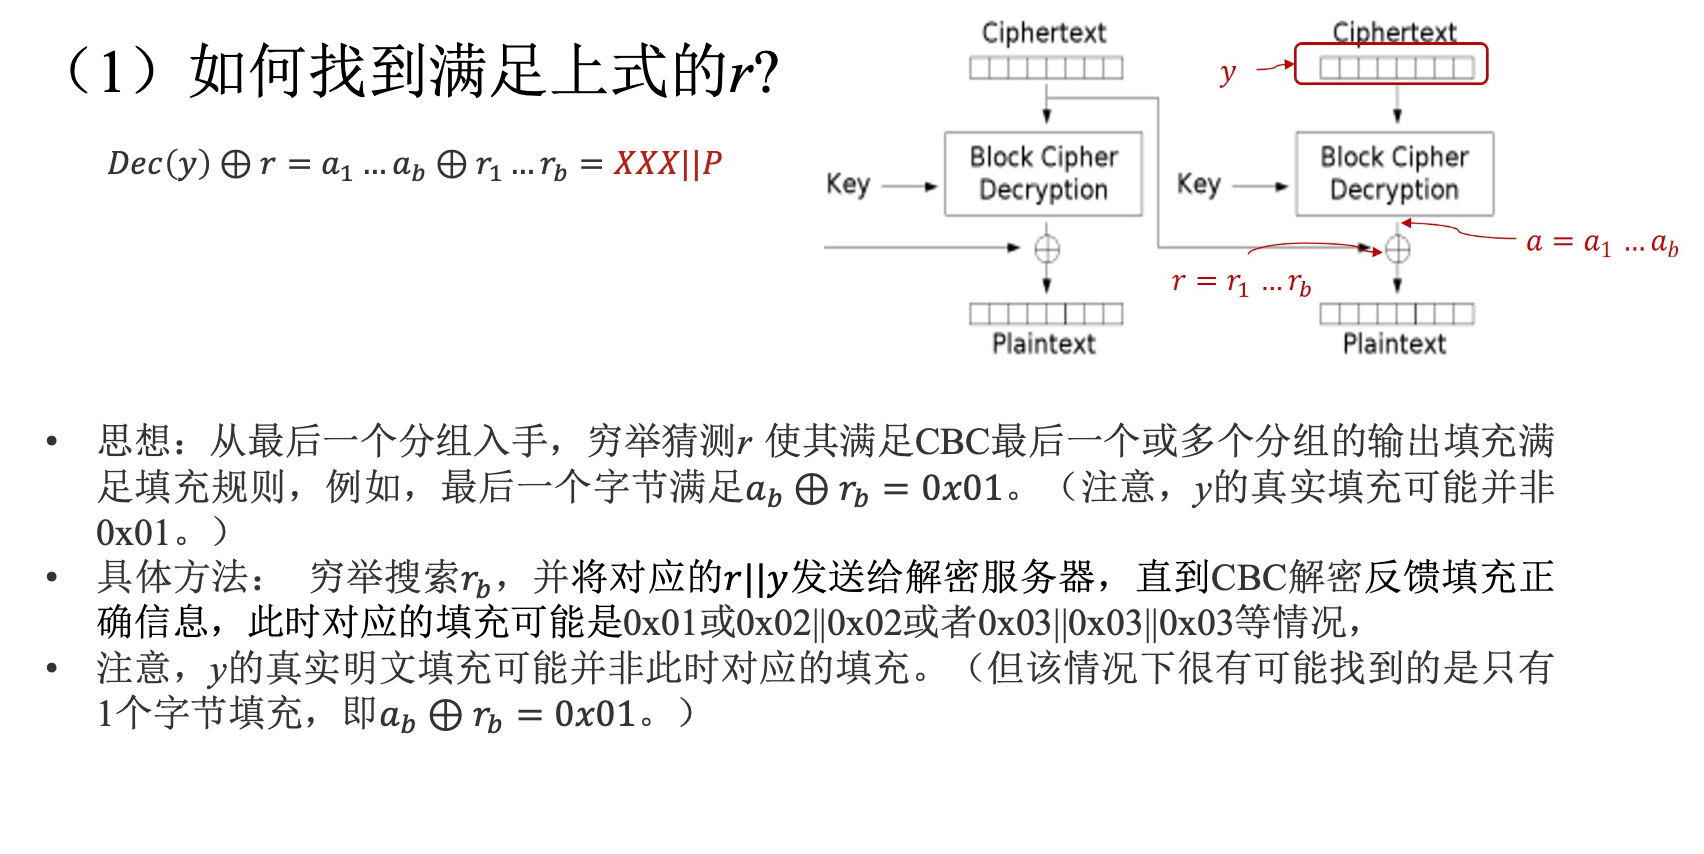
\includegraphics[width = 0.8\textwidth]{figures/error2.png}
    \caption{错误2}
\end{figure}
正如前面实验原理部分所说，在恢复最后一块时，这个步骤是没有必要的。
